% ta med damping på DP-delle

\documentclass[aspectratio=169,xcolor=dvipsnames]{beamer}
%\usetheme{SimplePlus}

\usepackage{hyperref}
\usepackage{graphicx} % Allows including images
\usepackage{booktabs} % Allows the use of \toprule, \midrule and \bottomrule in tables

%----------------------------------------------------------------------------------------
%	TITLE PAGE
%----------------------------------------------------------------------------------------

\title[PLS]{PLS IO koblinger} % The short title appears at the bottom of every slide, the full title is only on the title page
%\subtitle{Subtitle}

\author[Fred-Olav] {Fred-Olav Mosdal}

\institute[Fagskolen Rogaland VGS] % Your institution as it will appear on the bottom of every slide, may be shorthand to save space

\date{\today} % Date, can be changed to a custom date


%----------------------------------------------------------------------------------------
%	PRESENTATION SLIDES
%----------------------------------------------------------------------------------------

\begin{document}
\begin{frame}
\titlepage
	$$\includegraphics[width=4cm]{../../Fagskolen/StyringDel1/Fagskolen.jpg}$$
\end{frame}
\section{Digitale PLS inn- og utganger (IO-er)}


\begin{frame}
	\frametitle{Styringssystemers tre deler}
	\begin{columns}
		\begin{column}{0.5\textwidth}
	\begin{itemize}
		\item Inngangsenheter
		\item styreenheter 
		\item utgangsenheter
	\end{itemize}
		\end{column}
		\begin{column}{0.5\textwidth}
	$$\includegraphics[width=1\textwidth]{../output/noGPLimages/pls01.png}$$
		\end{column}
	\end{columns}
\end{frame}


\begin{frame}
	\frametitle{PLS-ens opprinnelse}
	\begin{columns}
		\begin{column}{0.5\textwidth}
			Ble lansert som erstatning for relestyringer\\
			Opprinnelsen sees fremdeles i det mest vanlige programeringsspråket for PLS-er Ladder Logic Diagram
		\end{column}
		\begin{column}{0.5\textwidth}
	$$\includegraphics[width=1\textwidth]{../output/noGPLimages/Modicon 084.jpg}$$
			\url{https://www.engineering.com/programmable-logic-controllers-the-evolution-of-a-disruptive-technology/}
		\end{column}
	\end{columns}
\end{frame}


\begin{frame}
	\frametitle{Eksempler på PLS-er}
$$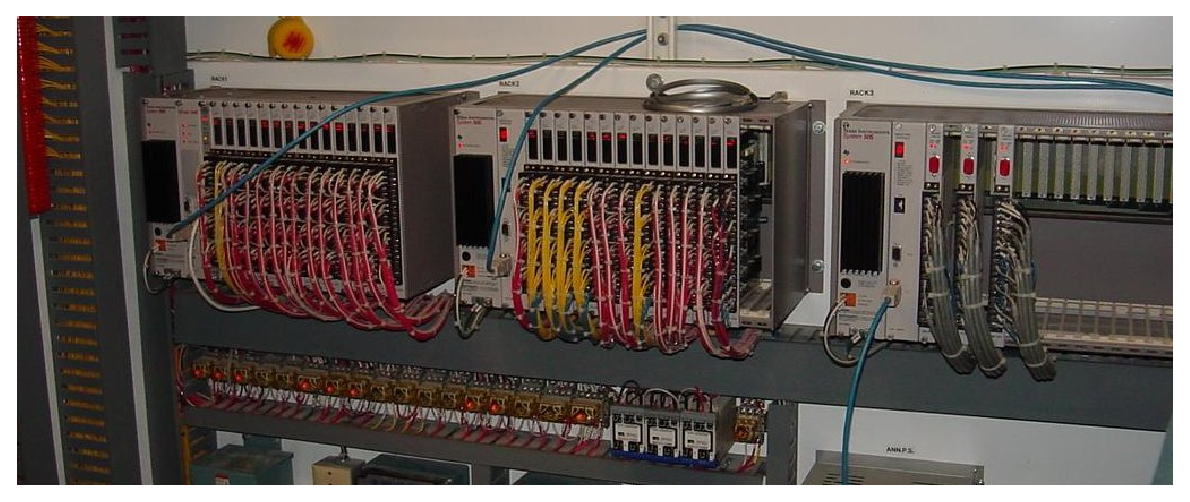
\includegraphics[width=1\textwidth]{plc_001.eps}$$
\end{frame}

\begin{frame}
	\frametitle{Eksempler på PLS-er}
$$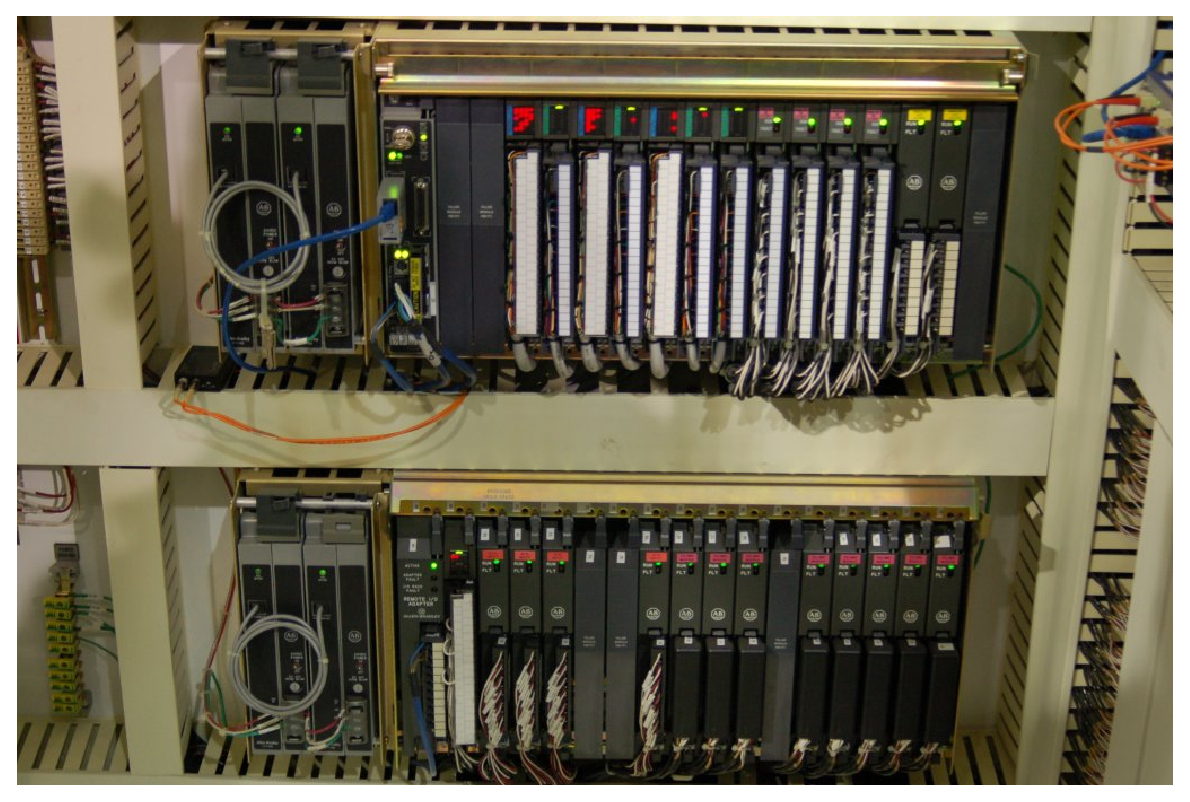
\includegraphics[width=0.8\textwidth]{plc_002.eps}$$
\end{frame}

\begin{frame}
	\frametitle{Eksempler på PLS-er}
$$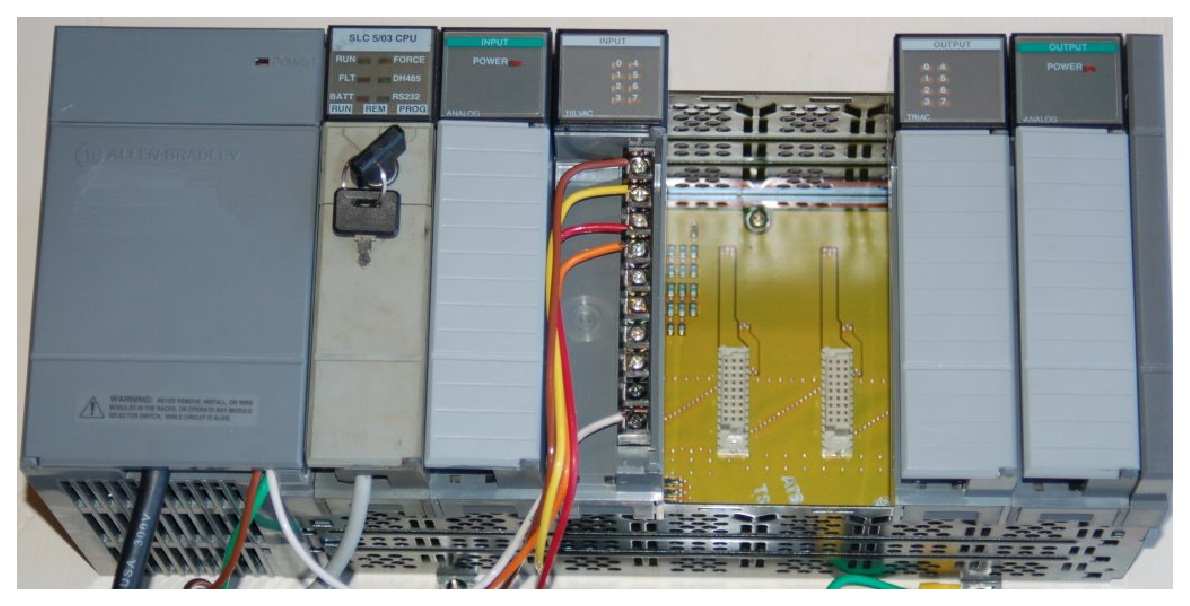
\includegraphics[width=0.9\textwidth]{plc_017.eps}$$
\end{frame}
\begin{frame}
	\frametitle{Eksempler på PLS-er}
$$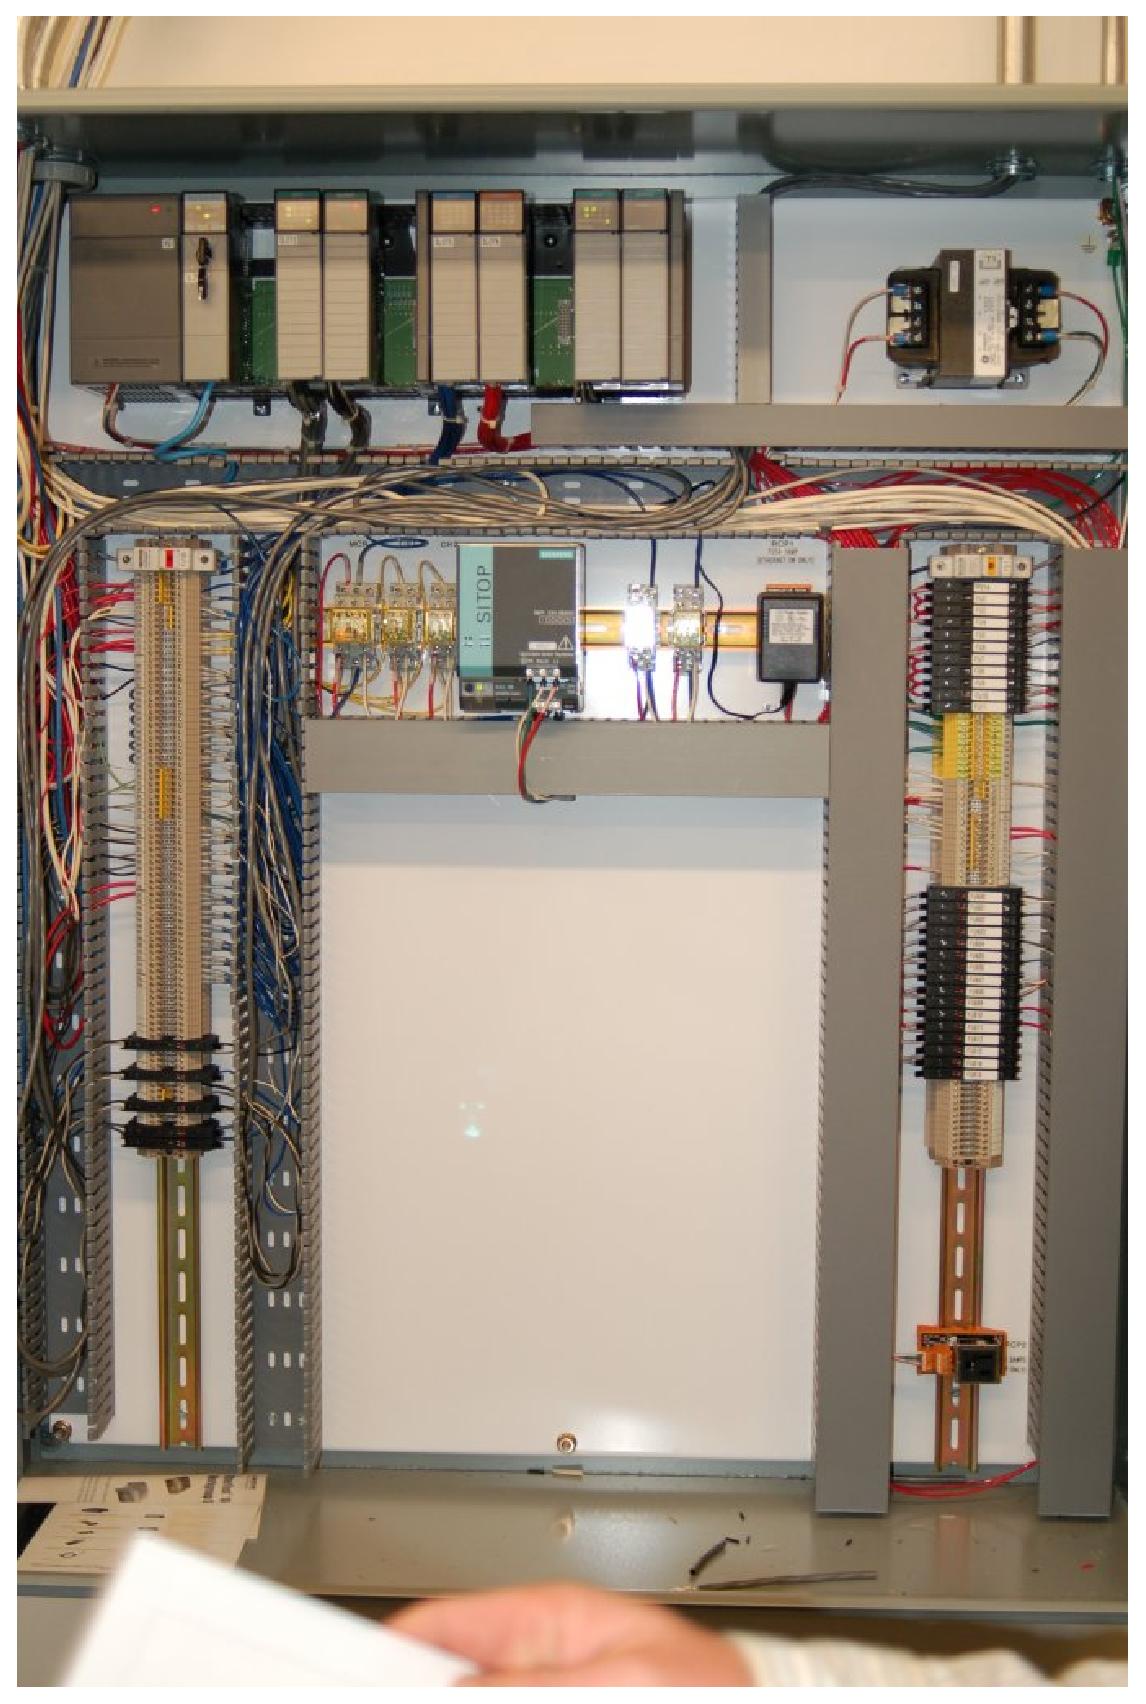
\includegraphics[width=0.8\textwidth]{plc_018.eps}$$
\end{frame}
\begin{frame}
	\frametitle{Eksempler på PLS-er}
$$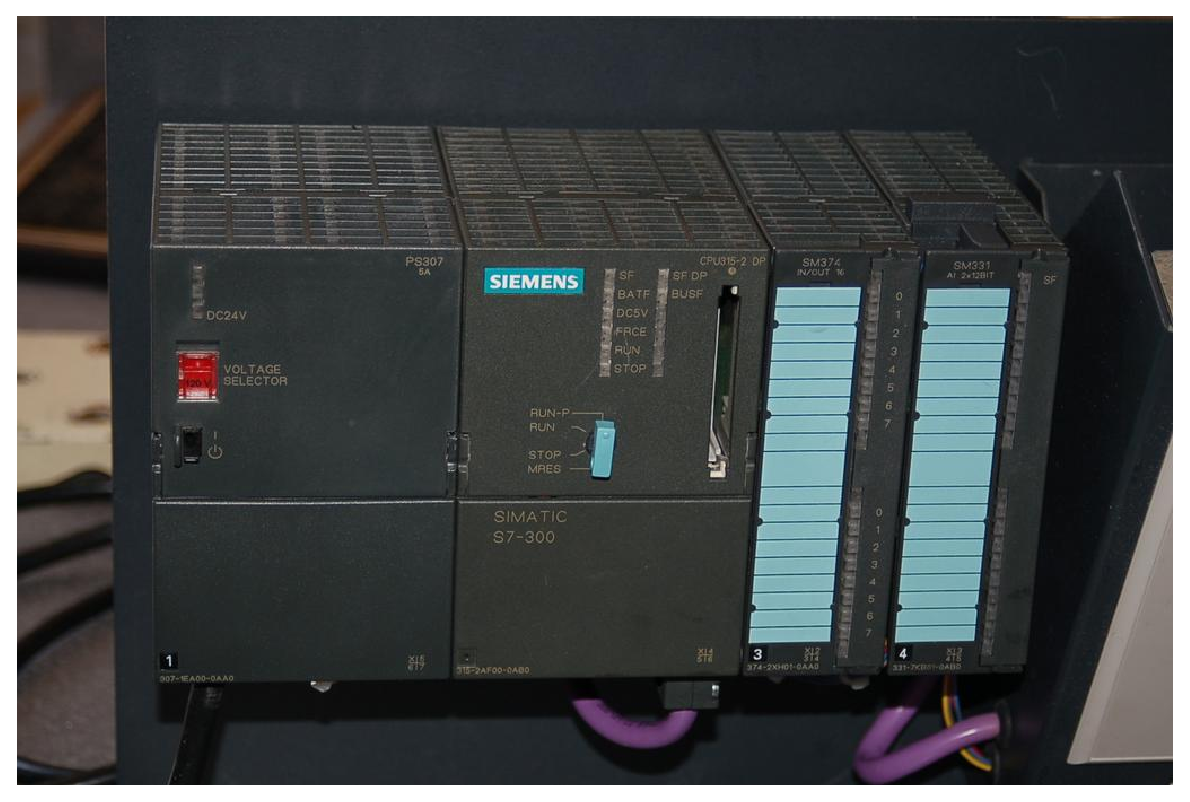
\includegraphics[width=0.7\textwidth]{plc_003.eps}$$
\end{frame}
\begin{frame}
	\frametitle{Eksempler på PLS-er}
$$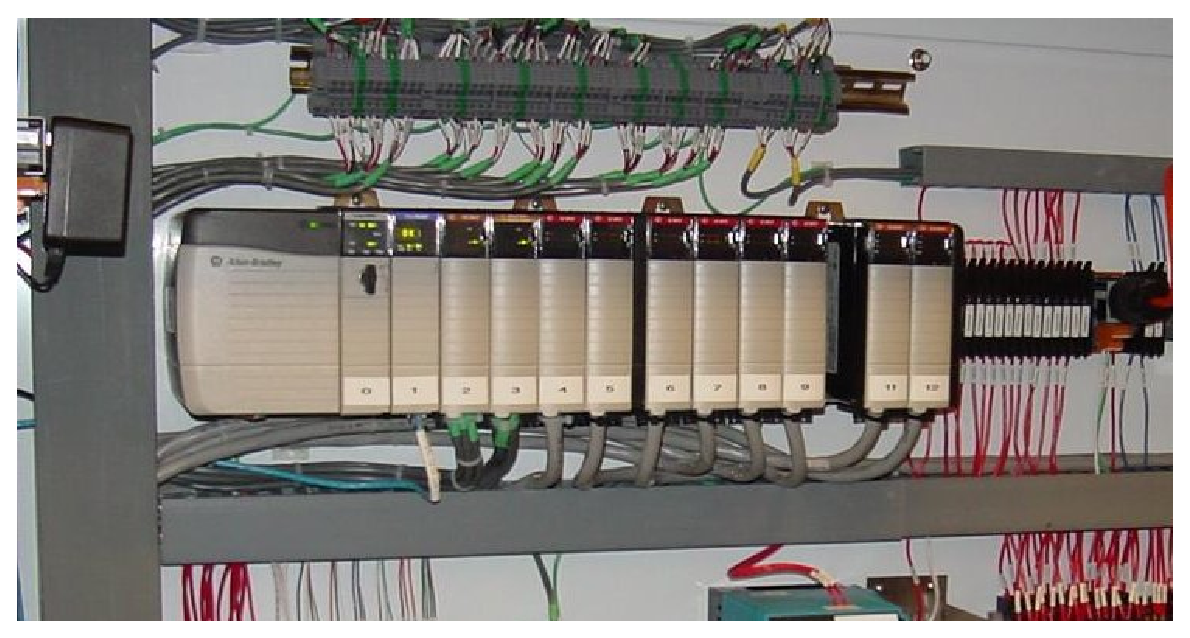
\includegraphics[width=0.9\textwidth]{plc_004.eps}$$
\end{frame}
\begin{frame}
	\frametitle{Eksempler på PLS-er}
$$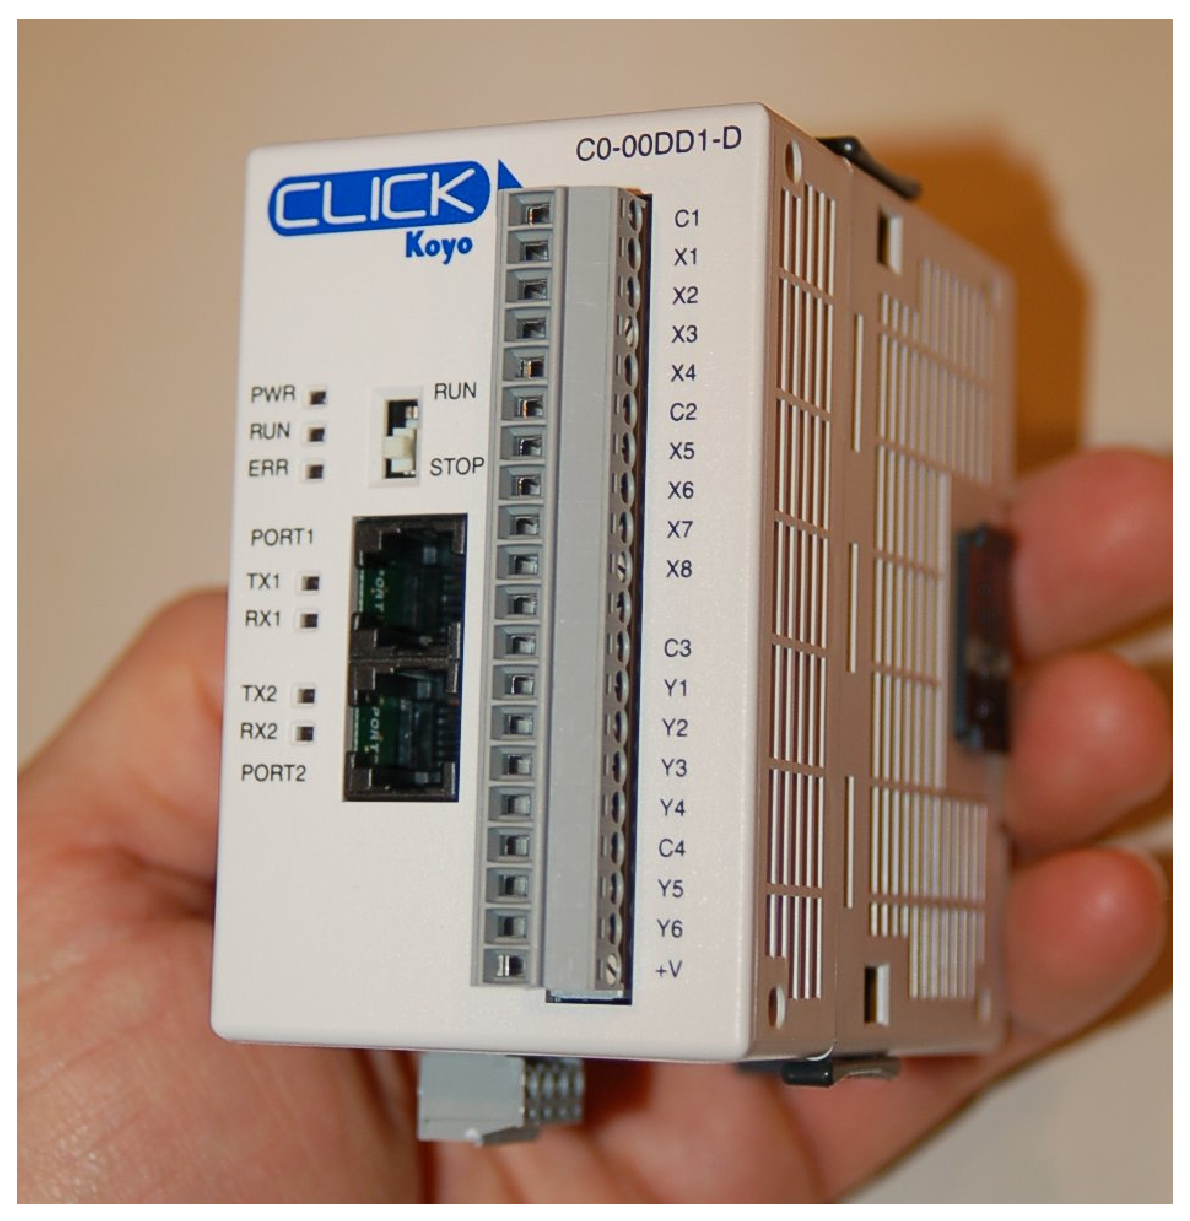
\includegraphics[width=0.5\textwidth]{plc_005.eps}$$
\end{frame}
\begin{frame}
	\frametitle{Eksempler på PLS-er}
$$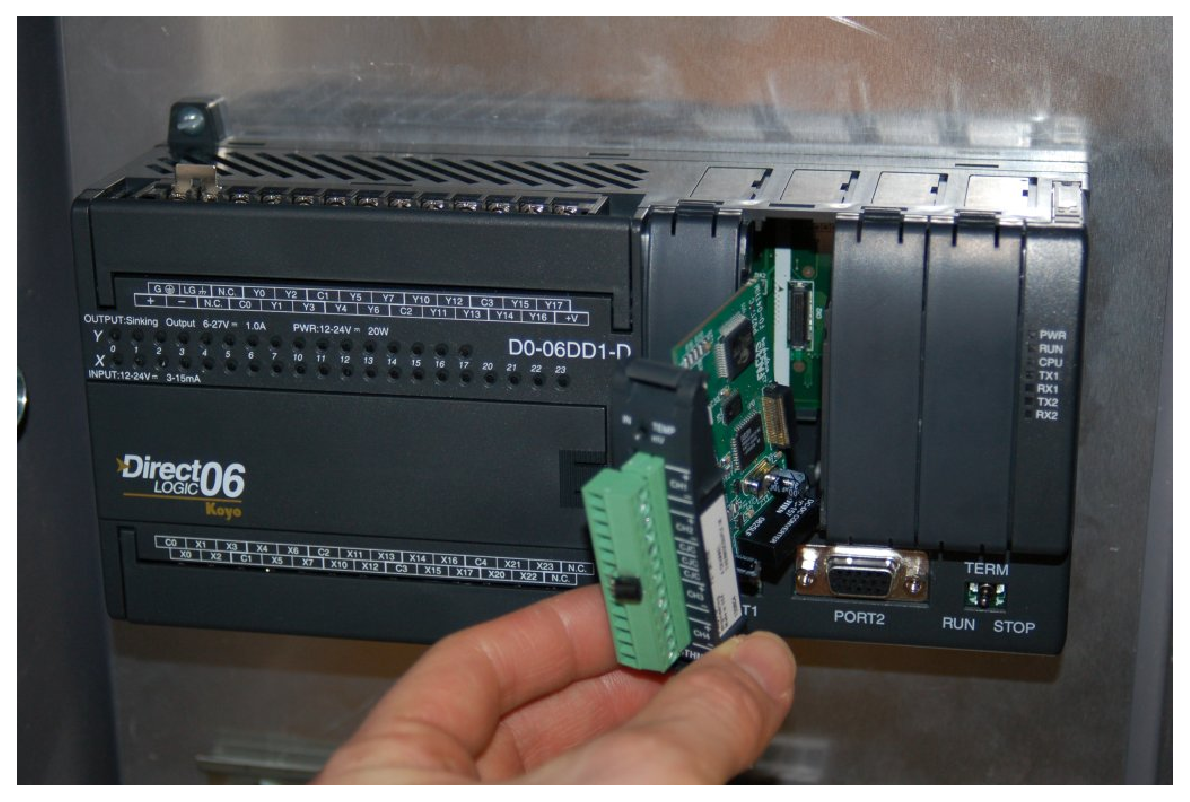
\includegraphics[width=0.8\textwidth]{plc_007.eps}$$
\end{frame}
\begin{frame}
	\frametitle{Eksempler på PLS-er}
$$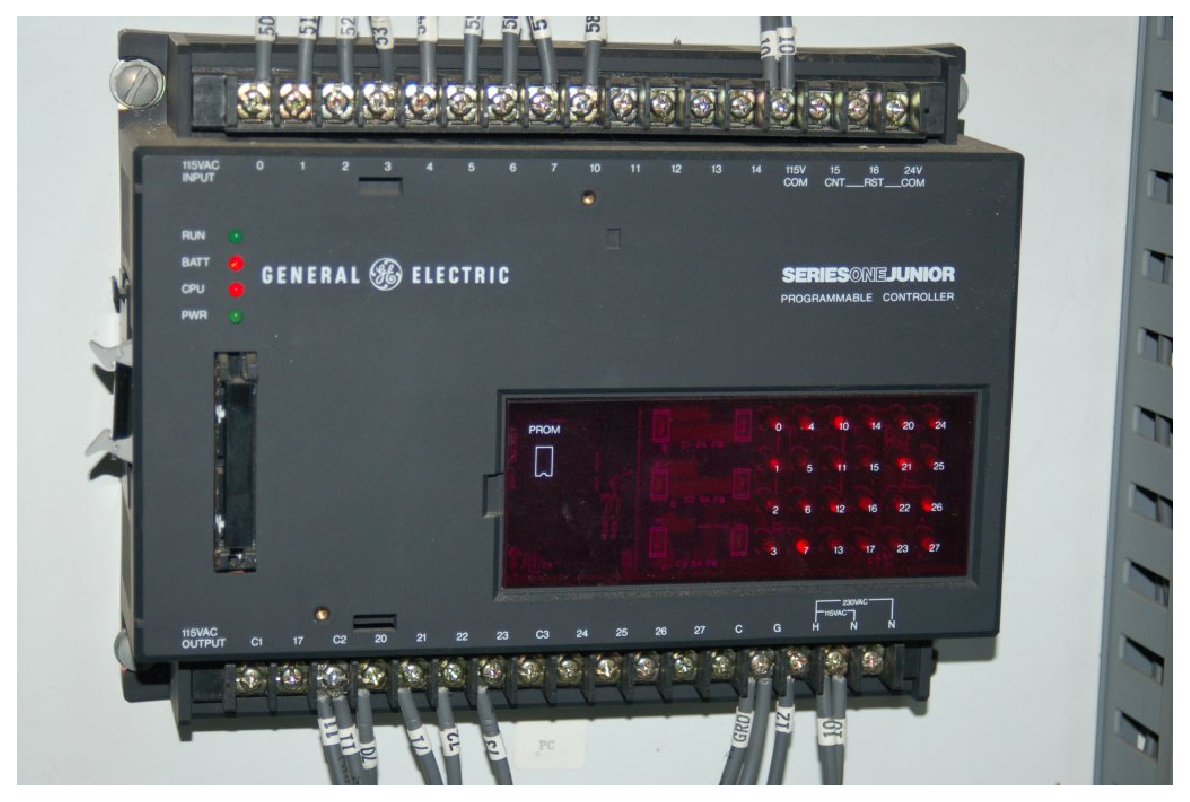
\includegraphics[width=0.8\textwidth]{plc_006.eps}$$
\end{frame}
\begin{frame}
	\frametitle{Inngangs- og utgangs tilkoblinger (IO-er)  }
	\framesubtitle{Tilgang til den virkelige verden}			
$$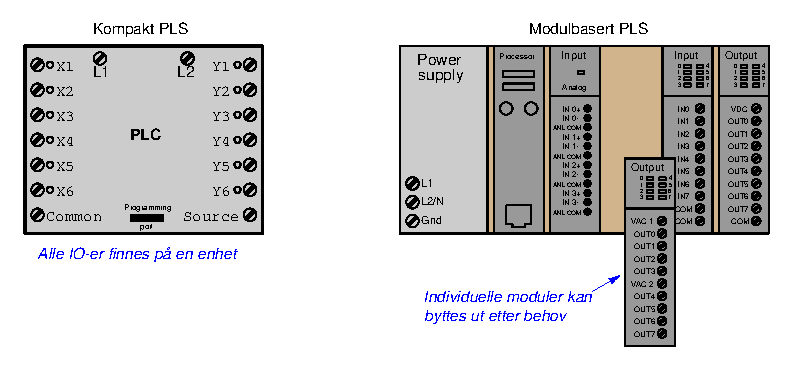
\includegraphics[width=0.8\textwidth]{plc_075.eps}$$
\end{frame}
\begin{frame}
	\frametitle{Inngangs- og utgangs tilkoblinger (IO-er)  }
	\framesubtitle{Tilgang til den virkelige verden}			
$$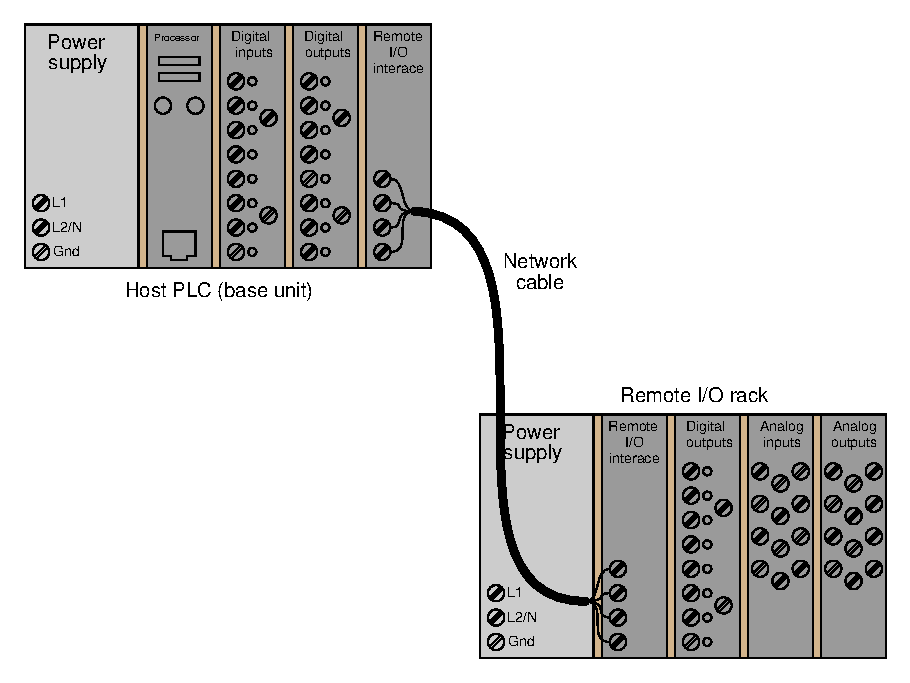
\includegraphics[width=0.6\textwidth]{plc_008.eps}$$
\end{frame}
\begin{frame}
	\frametitle{Galvaniske skiller}
	\begin{columns}
		\begin{column}{0.5\textwidth}
			\begin{itemize}
				\item \href{https://www.farnell.com/datasheets/73758.pdf}{\textbf{Isolerer}} PLS fra spenninger i felt. 
			\end{itemize}

			
		\end{column}

		\begin{column}{0.5\textwidth}
	$$\includegraphics[width=1\textwidth]{../output/noGPLimages/pls06.png}$$
		\end{column}
	\end{columns}
\end{frame}

\begin{frame}
	\frametitle{Digitale IO-er}
	\framesubtitle{Digital inngang}			
	Krav til PLS-IO er satt i \href{https://lese.standard.no/product/2503568/nb}{\textbf{NEK 61131-2}} --
	Eksempel på \href{https://www.ti.com/lit/ab/slla370d/slla370d.pdf}{\textbf{nyere inngang}}
$$\includegraphics[width=0.9\textwidth]{plc_073.eps}$$
\end{frame}

\begin{frame}
	\frametitle{Digitale IO-er}
	\framesubtitle{Digital utgang}			
$$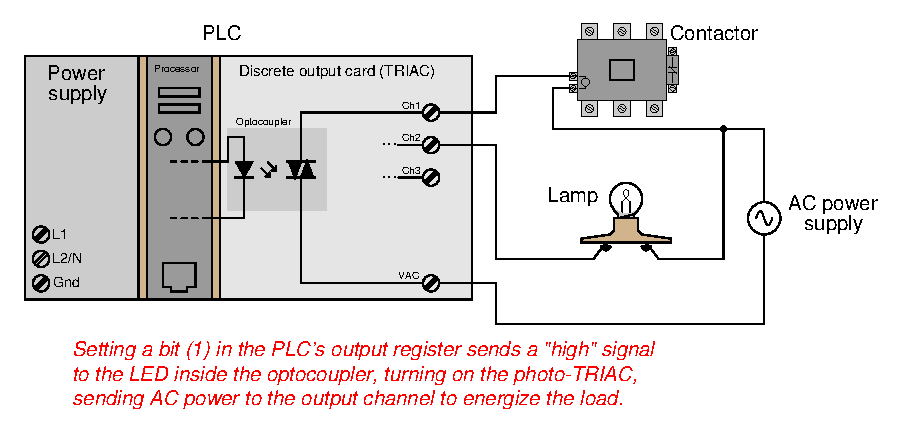
\includegraphics[width=0.9\textwidth]{plc_074.eps}$$
\end{frame}
\begin{frame}
	\frametitle{Sinking og Sourcing}
	\begin{columns}
		\begin{column}{0.5\textwidth}
		\begin{itemize}
			\item Inn- eller utgang som er sinking tar imot strøm 
			\item Inn- eller utgang som er soursing gir ut strøm 
		\end{itemize}	
		\end{column}
		\begin{column}{0.5\textwidth}

$$\includegraphics[width=0.9\textwidth]{plc_009.eps}$$
		\end{column}
	\end{columns}
\end{frame}


\begin{frame}
	\frametitle{Sinking og Sourcing}
	\begin{columns}
		\begin{column}{0.5\textwidth}
			
$$\includegraphics[width=0.9\textwidth]{plc_010.eps}$$
		\end{column}
		\begin{column}{0.5\textwidth}

$$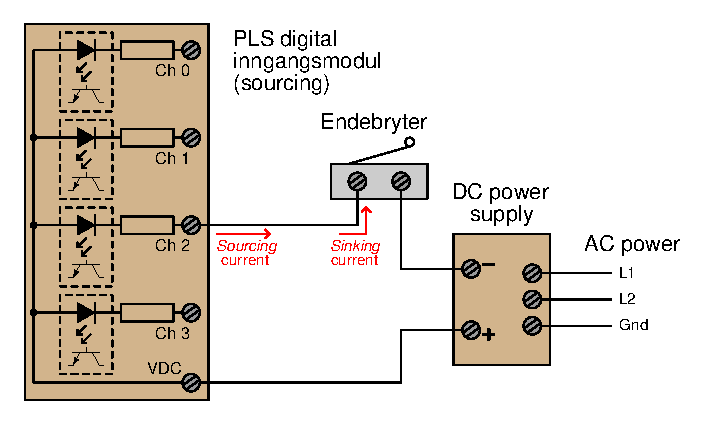
\includegraphics[width=0.9\textwidth]{plc_011.eps}$$
		\end{column}
	\end{columns}
\end{frame}
\begin{frame}
	\frametitle{Sinking og Sourcing}
	\begin{columns}
		\begin{column}{0.5\textwidth}
			
$$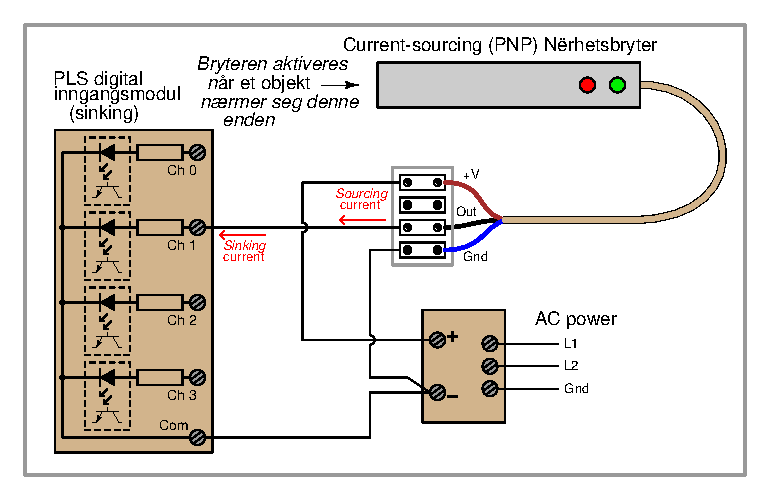
\includegraphics[width=1\textwidth]{plc_012_1.eps}$$
		\end{column}
		\begin{column}{0.5\textwidth}

$$\includegraphics[width=1\textwidth]{plc_012_2.eps}$$
		\end{column}
	\end{columns}
\end{frame}
\begin{frame}{Oppgave}
	\begin{columns}
		\begin{column}{0.3\textwidth}

			Hvilen er sinking og sourcring
			
		\end{column}

		\begin{column}{0.7\textwidth}
	$$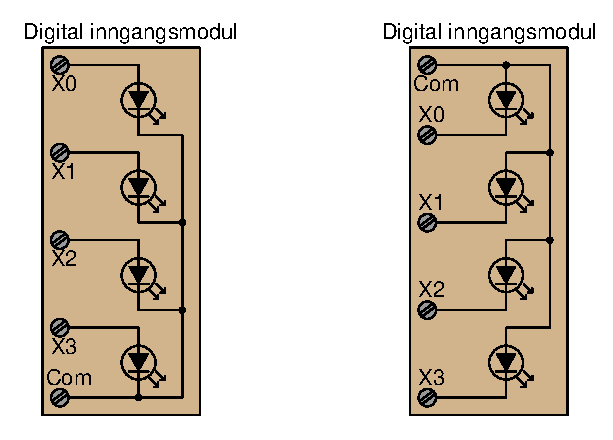
\includegraphics[height=0.8\textheight]{../src/i02359x01.eps}$$
		\end{column}
	\end{columns}
\end{frame}

\begin{frame}{Oppgave - 6ES7321-1BL00-0AA0}
	\begin{columns}
		\begin{column}{0.4\textwidth}

			Oppgaver: 
			\begin{itemize}
				\item Er dette en sinking eller sourcing PLS inngang 
				\item Tegn kobling for den øverste bryteren til inngang Ix0.4
				\item Tegn kobling for den nederste bryteren til inngang Ix0.7
			\end{itemize}
			
		\end{column}

		\begin{column}{0.6\textwidth}
			\href{https://docs.rs-online.com/4ccb/A700000009501908.pdf}{ 
			$$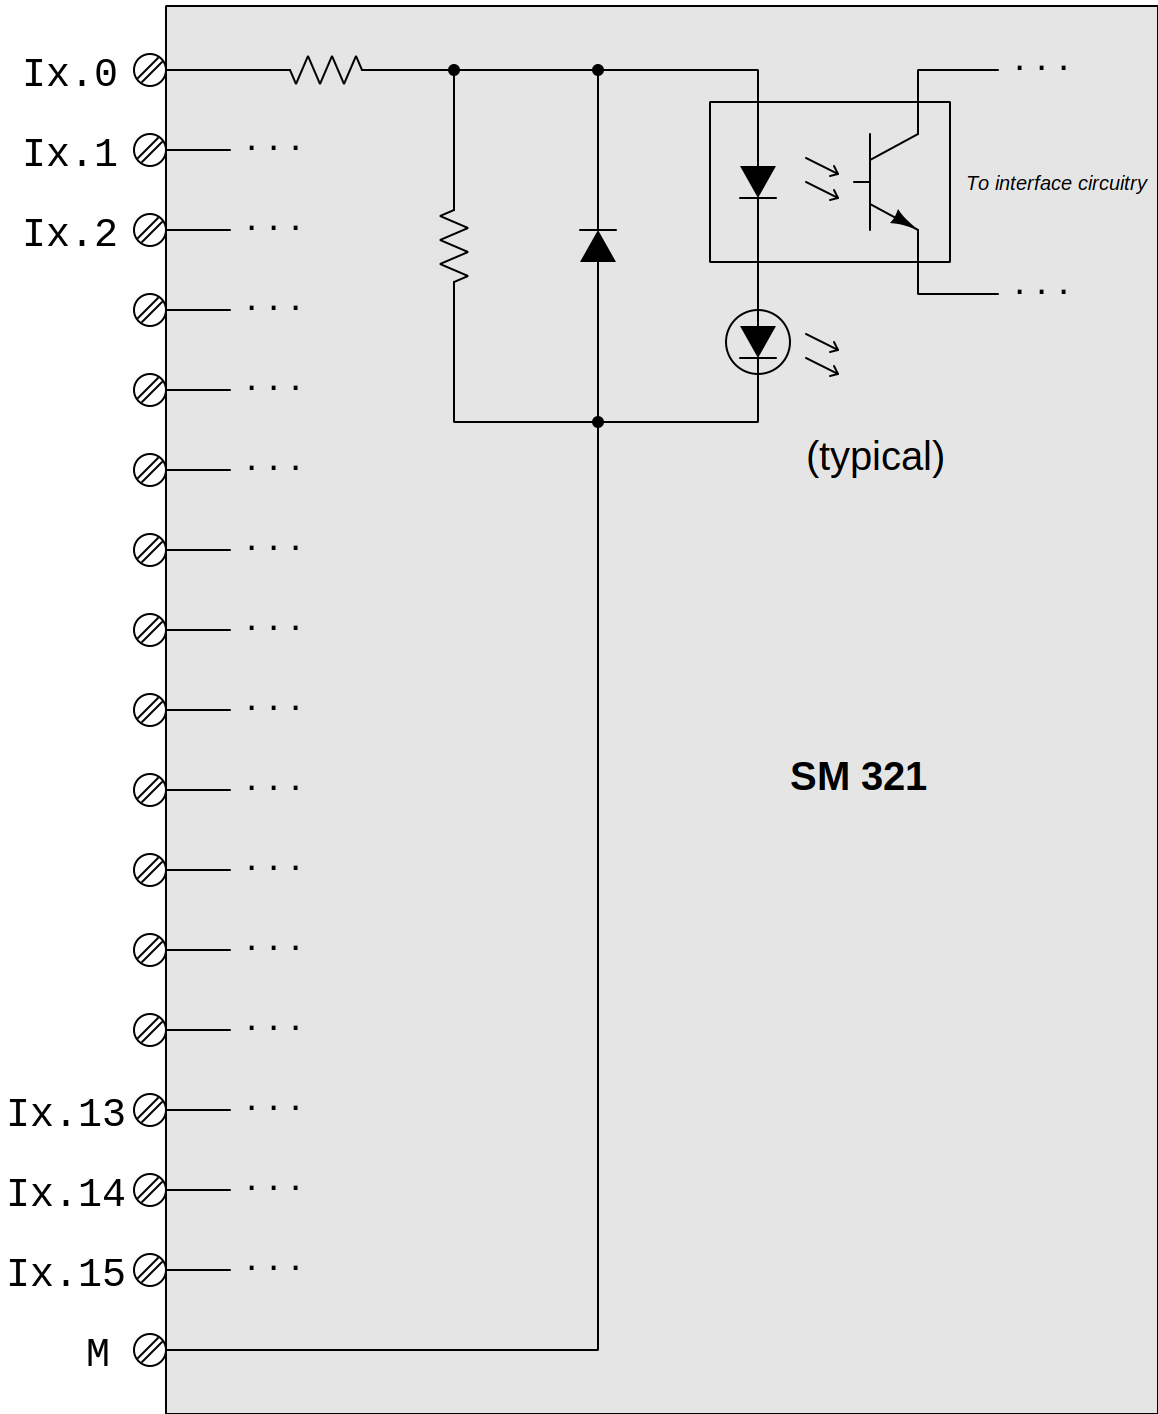
\includegraphics[height=0.8\textheight]{../src/i04536x01.eps}$$}
		\end{column}
	\end{columns}
\end{frame}
\begin{frame}{Oppgave}
	\begin{columns}
		\begin{column}{0.4\textwidth}

			Oppgaver: 
			\begin{itemize}
				\item Er dette en sinking eller sourcing PLS inngang 
				\item Tegn kobling for den øverste bryteren til inngang Ix0.4
				\item Tegn kobling for den nederste bryteren til inngang Ix0.7
			\end{itemize}
			
		\end{column}

		\begin{column}{0.6\textwidth}
	$$\includegraphics[height=0.8\textheight]{../src/i02508x01.eps}$$
		\end{column}
	\end{columns}
\end{frame}

\begin{frame}{Oppgave}
	\begin{columns}
		\begin{column}{0.4\textwidth}

			Oppgaver: 
			\begin{itemize}
				\item Hvilken koblings type har denne PLS-en
				\item Hvilken koblings type har denne sensoren
				\item Tegn kobling for den bryteren til inngang Ix0.5
			\end{itemize}
			
		\end{column}

		\begin{column}{0.6\textwidth}
	$$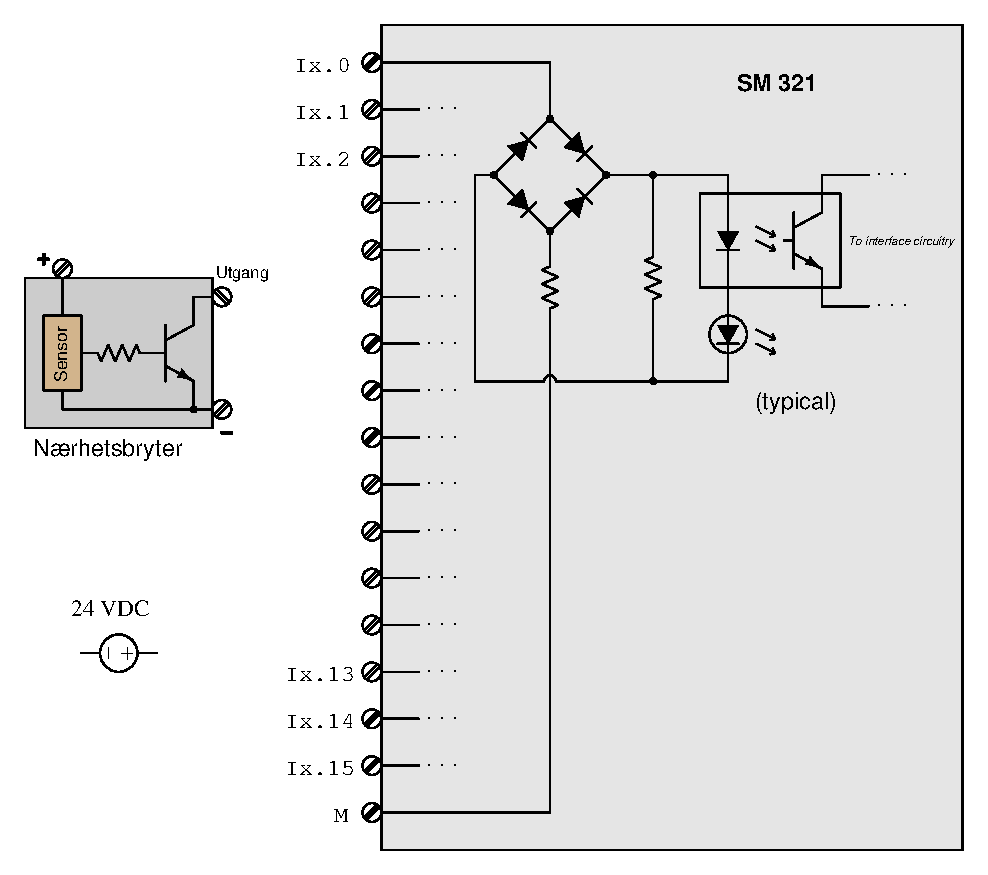
\includegraphics[height=0.8\textheight]{../src/i04544x01.eps}$$
		\end{column}
	\end{columns}
\end{frame}
\begin{frame}
	\frametitle{DO med rele}
	\begin{columns}
		\begin{column}{0.4\textwidth}
			Rele utganger :
			\begin{itemize}
				\item kan være potensialfrie
				\item Kan bryte forholdsvis store strømmer (6-10A)
				\item Kan brukes på AC og DC
			\end{itemize}

			
		\end{column}

		\begin{column}{0.6\textwidth}
	$$\includegraphics[height=0.6\textheight]{../output/noGPLimages/pls03.png}$$
		\end{column}
	\end{columns}
\end{frame}

\begin{frame}
	\frametitle{DO med transistor (Transistorutgang}
	\begin{columns}
		\begin{column}{0.5\textwidth}
			Transistorutganger:
			\begin{itemize}
				\item bryter mindre strømmer (0.5 og 1 A er vanlig)
				\item bryter raskere en rele utganger
				\item Finnes i NPN eller PNP utgaver
				\item NPN kalles også low side switching
				\item PNP kalles også high side switching
				\item Kan brukes på DC
			\end{itemize}

			
		\end{column}

		\begin{column}{0.5\textwidth}
	$$\includegraphics[width=1\textwidth]{../output/noGPLimages/pls04.png}$$
		\end{column}
	\end{columns}
\end{frame}

\begin{frame}
	\frametitle{DO med triac}
	\begin{columns}
		\begin{column}{0.5\textwidth}
			\begin{itemize}
				\item Kan bryte mindre AC strømmer en releer
				\item Tåler flere bryte sykluser
			\end{itemize}

			
		\end{column}

		\begin{column}{0.5\textwidth}
	$$\includegraphics[width=0.8\textwidth]{../output/noGPLimages/pls05.png}$$
		\end{column}
	\end{columns}
\end{frame}

\begin{frame}{Oppgave}
	\begin{columns}
		\begin{column}{0.4\textwidth}

			Oppgaver: 
			\begin{itemize}
				\item Hvilken oppgave har dioden på releet?
				\item Hvilken oppgave har dioden parallellt med utgangstransistoren?
				\item Hvilken oppgave har dioden i serie med optokobleren?
				\item Er det en sinking eller sourcsing PLS utgang?
				\item Tegn kobling som er nødvendig for å få releet til å virke 
			\end{itemize}
			
		\end{column}

		\begin{column}{0.6\textwidth}
	$$\includegraphics[height=0.8\textheight]{../src/i04537x01.eps}$$
		\end{column}
	\end{columns}
\end{frame}

\begin{frame}{Oppgave}
	\begin{columns}
		\begin{column}{0.4\textwidth}

			Oppgaver: 
			\begin{itemize}
				\item Tegn kobling for releet til Qx.5 
				\item Tegn kobling for solonoiden til Qx.7
			\end{itemize}
			
		\end{column}

		\begin{column}{0.6\textwidth}
	$$\includegraphics[height=0.8\textheight]{../src/i04246x01.eps}$$
		\end{column}
	\end{columns}
\end{frame}

\begin{frame}{Oppgave}
	Du skal koble opp PLS-en på neste slide. Koble til PSH som sinking sensor og PSL som sourcing sensor. Releene er 220V 
\end{frame}
\begin{frame}{Oppgave}
	$$\includegraphics[height=0.5\textheight]{../src/i02379x01.eps}$$
\end{frame}


\begin{frame}{Oppgave}
	Du skal koble opp PLS-en på neste slide. SSR-ene skal ha 24V
\end{frame}
\begin{frame}{Oppgave}
	$$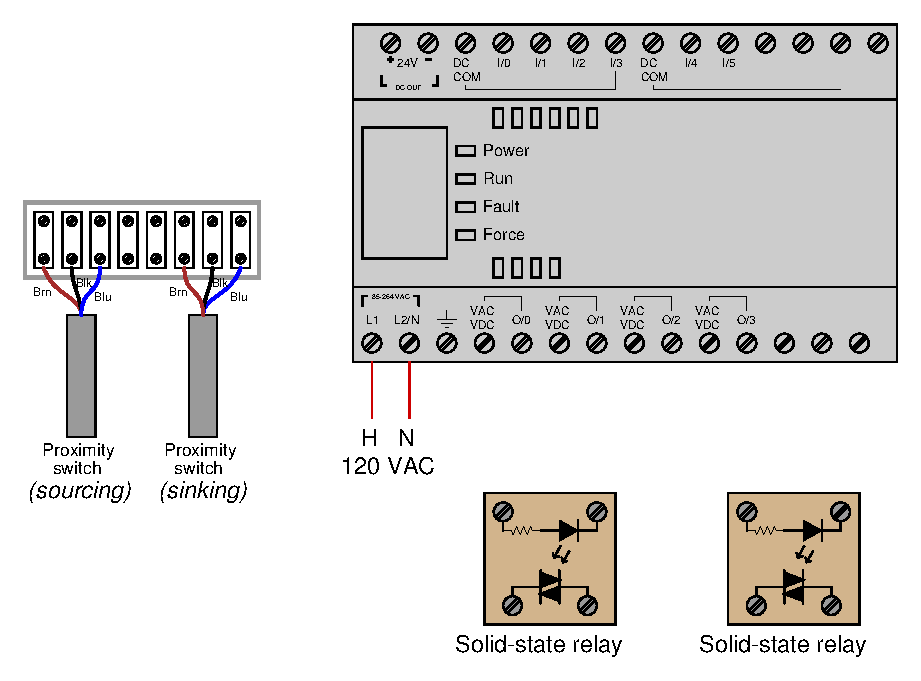
\includegraphics[height=0.7\textheight]{../src/i04524x01.eps}$$
\end{frame}
\begin{frame}{Oppgave}

			Anta at du har fått i oppdrag å koble disse tre trykkbrterene til DI-ene IN-4, IN-6 og IN-13 på en Allen-Bradley model 1756-IA16. Se neste slide. 
			
Tegn inn de nødvendige koblingene for at trykkbryterene skal virke på de spesifiserte DI-ene. Ta med eventuelt nødvendige spenningskilder. 
	Tips: Det kan hjelpe deg om du søker opp et dokument som kalles \href{https://literature.rockwellautomation.com/idc/groups/literature/documents/td/1756-td002_-en-e.pdf}{ \textbf{``1756 ControlLogix I/O Modules''}(publication 1756-TD002A-EN-E, May 2009)}
\end{frame}
\begin{frame}{Oppgave}
$$\includegraphics[width=10cm]{../src/i02060x01.eps}$$
\end{frame}

\end{document}
